\begin{figure}[t]
\begin{centering}
    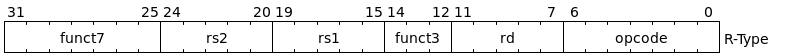
\includegraphics[width = \textwidth]{figures/Encoding-Types/R.png}\\
    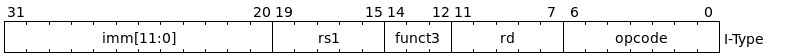
\includegraphics[width = \textwidth]{figures/Encoding-Types/I.png}\\
    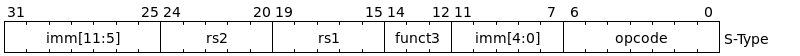
\includegraphics[width = \textwidth]{figures/Encoding-Types/S.png}\\
    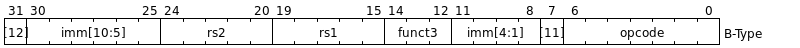
\includegraphics[width = \textwidth]{figures/Encoding-Types/B.png}\\
    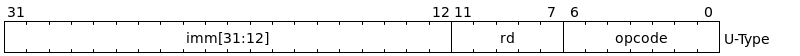
\includegraphics[width = \textwidth]{figures/Encoding-Types/U.png}\\
    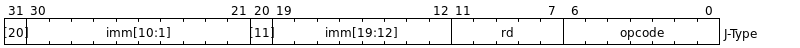
\includegraphics[width = \textwidth]{figures/Encoding-Types/J.png}
    \caption[RV64I encoding formats]{RV64I encoding formats, used in \cite{riscv-isa}(Chapter 2.3) \todo{Kopie richtig angeben}}
    \label{fig:rv64i_formats}
\end{centering}
\end{figure}
